\documentclass[conference]{IEEEtran}
\IEEEoverridecommandlockouts
\usepackage{cite}
\usepackage{amsmath,amssymb,amsfonts}
\usepackage{graphicx}
\usepackage{xcolor}
\usepackage{booktabs}
\usepackage{hyperref}
\usepackage{multirow}
\usepackage{tikz}
\usetikzlibrary{shapes,arrows,positioning,fit,backgrounds,calc,shadows}

\begin{document}

\title{Dual-Innovation Neural-Kalman Fusion for Real-Time Indoor Localization}

\author{
\IEEEauthorblockN{Utkarsh Agrawal\textsuperscript{*}\IEEEauthorrefmark{1},
Jayendra Vijay Birhade\textsuperscript{*}\IEEEauthorrefmark{1},
Neel Kanth Kundu\IEEEauthorrefmark{2}}
\IEEEauthorblockA{\IEEEauthorrefmark{1}Department of Computer Science and Engineering,
Indian Institute of Technology Delhi, New Delhi, India}
\IEEEauthorblockA{\IEEEauthorrefmark{2}Centre for Applied Research in Electronics,
Indian Institute of Technology Delhi, New Delhi, India\\
Email: neelkanth@iitd.ac.in}
\thanks{\textsuperscript{*}These authors contributed equally to this work.}
}

\maketitle

\begin{abstract}
Indoor positioning using hybrid smartphone sensors (Wi-Fi, Magnetic, and IMU) has seen growing interest, but deep-learning models often struggle to generalize in real-world deployments. This paper identifies key limitations in current regression methods, such as trajectory memorization, body-frame magnetic direction dependency, and non-causal look-ahead bias. To address these issues, we propose a generalized, decoupled, and strictly causal Neural-Kalman fusion framework for hybrid indoor localization. The architecture enforces a mathematical separation between spatial measurement extraction and temporal motion estimation. A Multi-Layer Perceptron (MLP) environment model maps dense Wi-Fi fingerprints from any $N$ Access Points to a 2D probability heatmap over $M$ discrete nodes. Simultaneously, a 1D Convolutional Neural Network (CNN) matches rotation-invariant magnetic sequences to structural anomaly maps. These spatial estimates are fused with a Pedestrian Dead Reckoning (PDR) motion model using an extended KalmanNet framework. The system replaces the fixed linear-Gaussian gain with dual $2\times2$ matrix gains dynamically produced by a Gated Recurrent Unit (GRU), utilizing availability masks to operate seamlessly even when only a subset of sensors is available. Evaluated rigorously on continuous real-world trajectories, the generalized system attains an error of 0.47~m under standard conditions and 1.07~m during degraded Wi-Fi scenarios, representing a 25.3\% improvement over single-innovation baselines.
\end{abstract}

\begin{IEEEkeywords}
Indoor positioning, Extended Kalman Filter, KalmanNet, sensor fusion, pedestrian dead reckoning, hybrid sensors.
\end{IEEEkeywords}

\section{Introduction}

Indoor localization is a critical technology for location-based services, smart buildings, and emergency navigation \cite{radar}. Because satellite signals attenuate severely indoors, systems must rely on ambient multi-modal smartphone sensors, primarily Wi-Fi Received Signal Strength Indication (RSSI), geomagnetic data, and Inertial Measurement Units (IMUs) \cite{horus, hybridwifi}. These signals are highly complementary: Wi-Fi offers absolute but infrequent position fixes, while IMU dead reckoning gives smooth, high-rate motion updates but suffers from cumulative drift \cite{nnwifipdr}. The geomagnetic field, meanwhile, presents a ubiquitous and stable distortion pattern inside modern steel-reinforced buildings, providing a dense source of structural context \cite{overviewdatasets}.

The fundamental challenge in hybrid indoor localization is developing a unified model that optimally fuses these discrete modalities while retaining robustness to sensor outages. Recent methodologies treat positioning as an end-to-end regression problem, utilizing Convolutional Neural Networks (CNNs) and Bidirectional Long Short-Term Memory networks (Bi-LSTMs) to map sequences directly to Cartesian coordinates \cite{deeppos,minloc, bilstmmag}. Advanced topological approaches have also utilized Graph Neural Networks (GNNs) \cite{wang2024gnn}, and virtual mapping techniques have attempted to generalize across physical structures \cite{rizk2023globloc}. However, standard sequence models possess critical limitations in live environments: they frequently memorize specific spatial routes rather than generalizing the environment, they suffer from heading-bias if raw body-frame magnetic vectors are used, and bidirectional architectures are fundamentally non-causal.

To address these limitations, we propose a generalized, decoupled, strictly causal Neural-Kalman fusion architecture designed for hybrid localization. Our framework separates spatial environment learning from temporal tracking. We construct generic models for any number of Wi-Fi Access Points ($N$) and spatial reference nodes ($M$), allowing broad applicability. Spatial updates are fused with a classical Pedestrian Dead Reckoning (PDR) model using a dual-innovation KalmanNet \cite{kalmannet}, which calculates context-dependent trust matrices dynamically and natively handles missing sensor modalities via input availability masks. 

The remainder of this paper is structured as follows. Section \ref{sec:architecture} mathematically formalizes the proposed generalized system architecture. Section \ref{sec:setup} details the experimental setup, dataset processing, and augmentation. Section \ref{sec:results} presents the performance evaluation, and Section \ref{sec:conclusion} concludes the paper.

\section{Proposed System Architecture}\label{sec:architecture}

Our proposed architecture functions as a modular, learned Bayesian filter designed for general hybrid indoor environments. It relies entirely on past and present observations, maintaining strict causality. The complete system architecture is illustrated in Fig.~\ref{fig:arch_diagram}.

\begin{figure}[htbp]
\centering
\resizebox{\columnwidth}{!}{
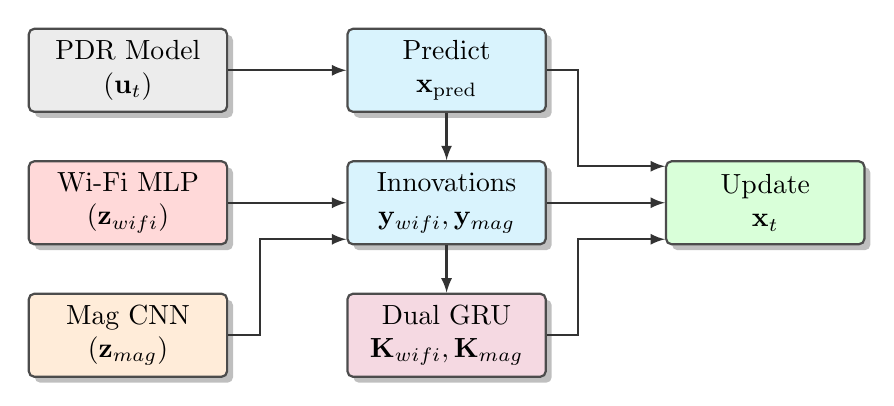
\begin{tikzpicture}[
    block/.style={rectangle, draw=black!70, thick, fill=blue!10, text width=6.5em, text centered, rounded corners=2pt, minimum height=3em, drop shadow},
    line/.style={draw, -latex, thick, color=black!80}
]
    % Sensors / Measurements
    \node [block, fill=gray!15] (pdr) {PDR Model \\ ($\mathbf{u}_t$)};
    \node [block, fill=red!15, below=0.6cm of pdr] (wifi) {Wi-Fi MLP \\ ($\mathbf{z}_{wifi}$)};
    \node [block, fill=orange!15, below=0.6cm of wifi] (mag) {Mag CNN \\ ($\mathbf{z}_{mag}$)};
    
    % KF Steps
    \node [block, fill=cyan!15, right=1.5cm of pdr] (predict) {Predict \\ $\mathbf{x}_{\text{pred}}$};
    \node [block, fill=cyan!15, right=1.5cm of wifi] (innov) {Innovations \\ $\mathbf{y}_{wifi}, \mathbf{y}_{mag}$};
    \node [block, fill=purple!15, right=1.5cm of mag] (gru) {Dual GRU \\ $\mathbf{K}_{wifi}, \mathbf{K}_{mag}$};
    
    \node [block, fill=green!15, right=1.5cm of innov] (update) {Update \\ $\mathbf{x}_t$};
    
    % Routing
    \path [line] (pdr) -- (predict);
    
    \path [line] (wifi) -- (innov);
    \path [line] (mag.east) -- ++(0.4,0) |- (innov.200); % Routes mag into innovations
    
    \path [line] (predict) -- (innov);
    \path [line] (innov) -- (gru);
    
    \path [line] (gru.east) -- ++(0.4,0) |- (update.200);
    \path [line] (innov) -- (update);
    \path [line] (predict.east) -- ++(0.4,0) |- (update.160);
\end{tikzpicture}
}
\caption{The proposed Neural-Kalman Fusion Architecture. Both the Wi-Fi probability heatmap and the continuous 1D-CNN magnetic fix generate innovations against the PDR prediction. A recurrent Dual GRU observes these innovations to compute optimal Kalman gain matrices for the state update.}
\label{fig:arch_diagram}
\end{figure}

\subsection{General Problem Formulation}
Assume a targeted indoor environment characterized by $N$ uniquely identifiable Wi-Fi Access Points (APs) and a discrete reference grid containing $M$ surveyed spatial nodes (Reference Points). At any discrete time step $t$, the smartphone yields a subset of sensory data: an IMU vector sequence (acceleration and gyroscope), a 3D magnetic field vector $\mathbf{M}_t \in \mathbb{R}^3$, and a sparsely sampled Wi-Fi RSSI vector $\mathbf{s}_t \in \mathbb{R}^N$. Our objective is to continuously estimate the user's 2D Cartesian spatial state $\mathbf{x}_t = [x_t, y_t]^T \in \mathbb{R}^2$.

\subsection{Wi-Fi Processing and Heatmap Model}

The Wi-Fi scan $\mathbf{s}_t$ is normalized into $\mathbf{x}_{wifi} \in [0,1]^N$ by clipping to [-90, -30]~dBm and rescaling. Absent APs are assigned a constant floor value of $-100$~dBm. 

To map this highly non-linear signal to spatial coordinates, we employ a Multi-Layer Perceptron (MLP) with Dropout regularization ($p=0.3$). The MLP processes $\mathbf{x}_{wifi}$ and outputs a probability vector $\mathbf{p} \in \mathbb{R}^M$ over the discrete grid cells. 
\begin{figure}[htbp]
\centering
\resizebox{\columnwidth}{!}{
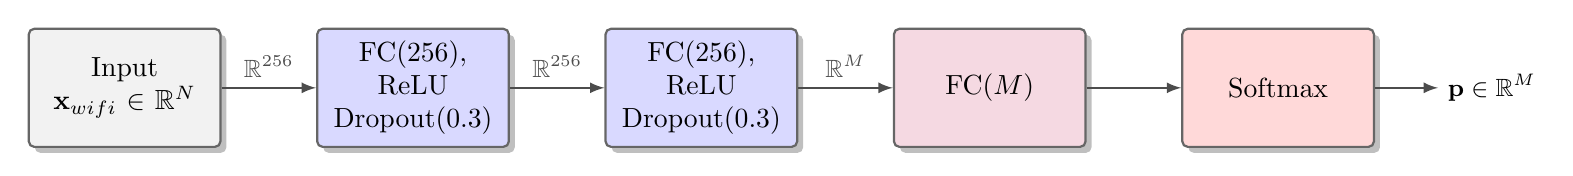
\begin{tikzpicture}[
    layer/.style={rectangle, draw=black!60, thick, fill=blue!10, text centered, rounded corners=2pt, minimum height=1.5cm, drop shadow, text width=2.2cm},
    arrow/.style={draw, thick, -latex, color=black!70},
    label/.style={font=\small\sffamily}
]
    % Nodes (Horizontal layout)
    \node[layer, fill=gray!10] (input) {Input\\$\mathbf{x}_{wifi} \in \mathbb{R}^N$};
    
    \node[layer, right=1.2cm of input, fill=blue!15] (fc1) {FC(256), ReLU\\Dropout(0.3)};
    \node[layer, right=1.2cm of fc1, fill=blue!15] (fc2) {FC(256), ReLU\\Dropout(0.3)};
    \node[layer, right=1.2cm of fc2, fill=purple!15] (fc3) {FC($M$)};
    
    \node[layer, right=1.2cm of fc3, fill=red!15] (softmax) {Softmax};
    \node[label, right=0.8cm of softmax] (output) {$\mathbf{p} \in \mathbb{R}^M$};

    % Arrows
    \path [arrow] (input) -- (fc1) node[midway, above, label] {$\mathbb{R}^{256}$};
    \path [arrow] (fc1) -- (fc2) node[midway, above, label] {$\mathbb{R}^{256}$};
    \path [arrow] (fc2) -- (fc3) node[midway, above, label] {$\mathbb{R}^{M}$};
    \path [arrow] (fc3) -- (softmax);
    \path [arrow] (softmax) -- (output);
\end{tikzpicture}
}
\caption{Architecture of the Wi-Fi Multi-Layer Perceptron (MLP) environment model. Dense layers sequentially extract features from the RSSI vector to compute an $M$-dimensional probability heatmap.}
\label{fig:mlp_arch}
\end{figure}

The training target is defined as a two-dimensional Gaussian probability distribution $\mathbf{q} \in \mathbb{R}^M$ centered precisely on the true coordinate of the surveyed node (with spatial standard deviation $\sigma = 2.0$~m). The network is optimized using the Kullback-Leibler (KL) divergence loss:
\begin{equation}
\mathcal{L}_{MLP} = D_{KL}(\mathbf{q} \parallel \mathbf{p}) = \sum_{c=1}^{M} q_c \log \left( \frac{q_c}{p_c} \right) \label{eq:kl_loss}
\end{equation}

During real-time inference, the continuous coordinate estimate $\mathbf{z}_{wifi}$ and the associated measurement covariance matrix $\mathbf{R}_{hm}$ are computed as the probability-weighted expectation (soft-argmax):
\begin{equation}
\mathbf{z}_{wifi} = \sum_{c=1}^{M} p_c \cdot \mathbf{C}_c \label{eq:heatmap_centroid}
\end{equation}
\begin{equation}
\mathbf{R}_{hm} = \sum_{c=1}^{M} p_c\,(\mathbf{C}_c - \mathbf{z}_{wifi})(\mathbf{C}_c - \mathbf{z}_{wifi})^T \label{eq:heatmap_cov}
\end{equation}
where $\mathbf{C}_c \in \mathbb{R}^2$ denotes the physical coordinates of grid cell $c$. A concentrated heatmap yields a tightly bounded covariance, providing an honest, per-scan confidence estimate to the downstream filter.

\subsection{Magnetic Sequence Matcher}

To mitigate orientation bias inherent in raw $\mathbf{M}_t$ vectors, we extract 4 rotation-invariant features per frame: the field magnitude $||\mathbf{M}_t||$, the vertical projection against estimated gravity, the horizontal component magnitude, and the magnetic dip angle. Because single-point magnetic matching is highly ambiguous, we utilize a 1D Convolutional Neural Network (CNN) to map a temporal sliding window (length $T$) of these 4-channel features to a spatial coordinate.

\begin{figure}[htbp]
\centering
\resizebox{\columnwidth}{!}{
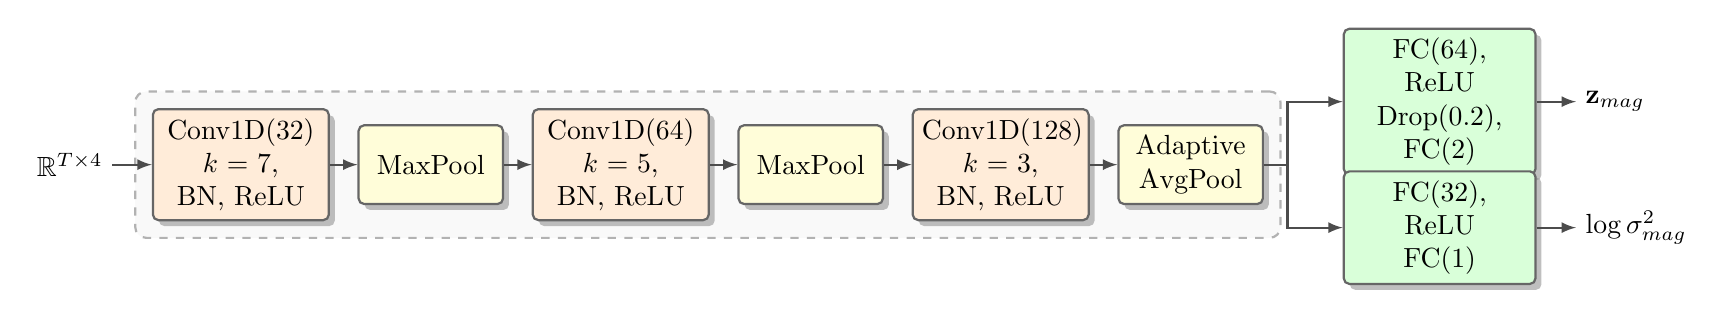
\begin{tikzpicture}[
    conv/.style={rectangle, draw=black!60, thick, fill=orange!15, text centered, rounded corners=2pt, minimum height=1cm, drop shadow, text width=2cm},
    pool/.style={rectangle, draw=black!60, thick, fill=yellow!15, text centered, rounded corners=2pt, minimum height=1cm, drop shadow, text width=1.6cm},
    head/.style={rectangle, draw=black!60, thick, fill=green!15, text centered, rounded corners=2pt, minimum height=1cm, drop shadow, text width=2.2cm},
    arrow/.style={draw, thick, -latex, color=black!70},
    groupbox/.style={rectangle, draw=black!30, dashed, thick, inner sep=6pt, rounded corners}
]
    % Input
    \node (input) {$\mathbb{R}^{T \times 4}$};
    
    % Encoder
    \node[conv, right=0.5cm of input] (conv1) {Conv1D(32)\\$k\!=\!7$, BN, ReLU};
    \node[pool, right=0.35cm of conv1] (pool1) {MaxPool};
    \node[conv, right=0.35cm of pool1] (conv2) {Conv1D(64)\\$k\!=\!5$, BN, ReLU};
    \node[pool, right=0.35cm of conv2] (pool2) {MaxPool};
    \node[conv, right=0.35cm of pool2] (conv3) {Conv1D(128)\\$k\!=\!3$, BN, ReLU};
    \node[pool, right=0.35cm of conv3] (gap) {Adaptive\\AvgPool};
    
    % Group Encoder
    \begin{scope}[on background layer]
        \node[groupbox, fill=gray!5, fit=(conv1) (gap)] (encoder_box) {};
    \end{scope}

    % Branching Heads
    \node[head, right=1cm of gap, yshift=0.8cm] (pos_head) {FC(64), ReLU\\Drop(0.2), FC(2)};
    \node[head, right=1cm of gap, yshift=-0.8cm] (var_head) {FC(32), ReLU\\FC(1)};
    
    % Outputs
    \node[right=0.5cm of pos_head] (outpos) {$\mathbf{z}_{mag}$};
    \node[right=0.5cm of var_head] (outvar) {$\log\sigma^2_{mag}$};

    % Connections
    \path [arrow] (input) -- (conv1);
    \path [arrow] (conv1) -- (pool1);
    \path [arrow] (pool1) -- (conv2);
    \path [arrow] (conv2) -- (pool2);
    \path [arrow] (pool2) -- (conv3);
    \path [arrow] (conv3) -- (gap);
    
    \draw [arrow] (gap.east) -- ++(0.3,0) |- (pos_head.west);
    \draw [arrow] (gap.east) -- ++(0.3,0) |- (var_head.west);
    
    \path [arrow] (pos_head) -- (outpos);
    \path [arrow] (var_head) -- (outvar);
    
\end{tikzpicture}
}
\caption{Architecture of the 1D-CNN Magnetic Sequence Matcher. A shared convolutional encoder with BatchNorm extracts temporal features, which are processed by two independent heads: a position head (with Dropout) predicting a 2D coordinate, and a variance head estimating heteroscedastic uncertainty.}
\label{fig:cnn_arch}
\end{figure}

The CNN processes the input to yield both a continuous position fix $\mathbf{z}_{mag} \in \mathbb{R}^2$ and a calibrated scalar log-variance $\log(\sigma^2_{mag})$. It is optimized using a heteroscedastic Negative Log-Likelihood (NLL) loss, which balances coordinate accuracy against self-reported confidence:
\begin{equation}
\mathcal{L}_{CNN} = \frac{1}{B} \sum_{i=1}^{B} \left( \frac{\| \mathbf{z}_{mag}^{(i)} - \mathbf{z}_{true}^{(i)} \|^2}{2\sigma^{2(i)}_{mag}} + \frac{1}{2}\log(\sigma^{2(i)}_{mag}) \right) \label{eq:nll_loss}
\end{equation}
where $B$ is the batch size, $\mathbf{z}_{true}$ is the ground-truth coordinate, and the variance $\sigma^2_{mag} = \exp(\text{logvar})$ is clamped to a minimum of 0.01 for numerical stability.

\subsection{Causal Pedestrian Dead Reckoning (PDR)}

The Pedestrian Dead Reckoning (PDR) system computes relative displacement at the full IMU rate. A step event is detected by applying a first-order exponential high-pass filter to the acceleration magnitude $\|\mathbf{a}_t\|$ (with smoothing factor $\alpha = 0.98$) and triggering when the residual exceeds an empirical threshold $\tau = 0.6$~m/s$^2$, subject to a refractory period of 0.3~s. The high-pass filter removes the static gravitational component ($\approx 9.81$~m/s$^2$), isolating the dynamic transients caused by foot impacts.

Upon detection, the discrete control displacement vector $\mathbf{u}_t$ is computed as:
\begin{equation}
\mathbf{u}_t = \begin{bmatrix} L_s \cos(\theta_t + \phi_h) \\ L_s \sin(\theta_t + \phi_h) \end{bmatrix} \label{eq:pdr}
\end{equation}
where $L_s$ is the calibrated step length (determined by matching integrated step count to ground-truth path length), $\theta_t$ is the real-time yaw heading angle from the device's orientation sensor at time $t$, and $\phi_h$ is the constant angular offset between the device's local orientation frame and the map's coordinate frame, calibrated as the mean angular difference between the device heading and the true trajectory direction over the training walks. 

\subsection{Dual-Innovation KalmanNet Fusion}\label{sec:kalmannet}

Classical EKFs rely on fixed covariance assumptions that fail to model highly variable multi-modal environments. We implement KalmanNet \cite{kalmannet}, replacing the analytical Kalman gain with a learned one computed by a Gated Recurrent Unit (GRU). The prediction step follows standard dead reckoning:
\begin{equation}
\mathbf{x}_{\text{pred}} = \mathbf{x}_{t-1} + \mathbf{u}_t \label{eq:kn_predict}
\end{equation}

The Wi-Fi innovation is a standard spatial residual:
\begin{equation}
\mathbf{y}_{wifi} = \mathbf{z}_{wifi} - \mathbf{x}_{\text{pred}} \in \mathbb{R}^2 \label{eq:kn_innovate_w}
\end{equation}

The magnetic innovation, however, operates in the scalar anomaly domain rather than Cartesian space. The observed magnetic anomaly value at the current position is compared to the pre-surveyed map value $A(\mathbf{x}_{\text{pred}})$:
\begin{equation}
y_{mag} = A_{\text{obs}} - A(\mathbf{x}_{\text{pred}}) \in \mathbb{R} \label{eq:kn_innovate_m}
\end{equation}

To convert this scalar mismatch into a 2D spatial correction, it is scaled by the spatial gradient $\nabla A = [\frac{\partial A}{\partial x}, \frac{\partial A}{\partial y}]^T$ of the pre-surveyed anomaly field, computed via discrete finite differences on the reference grid.

The input feature vector to the GRU encompasses 13 variables: the Wi-Fi innovation $\mathbf{y}_{wifi}$ (2), the scalar magnetic innovation $y_{mag}$ (1), the field gradient $\nabla A$ (2), the temporal difference of consecutive Wi-Fi fixes $\Delta \mathbf{z}_{wifi}$ (2), the PDR control $\mathbf{u}_t$ (2), the previous state update $\Delta \mathbf{x}_{t-1}$ (2), and two binary availability masks $m_{wifi}, m_{mag} \in \{0, 1\}$ (1+1).

The GRU outputs an 8-dimensional vector, reshaped into two independent $2\!\times\!2$ gain matrices, $\mathbf{K}_{wifi}$ and $\mathbf{K}_{mag}$. The posterior state $\mathbf{x}_t$ is updated as:
\begin{equation}
\mathbf{x}_t = \mathbf{x}_{\text{pred}} + m_{wifi} \cdot \mathbf{K}_{wifi} \mathbf{y}_{wifi} + m_{mag} \cdot \mathbf{K}_{mag} (y_{mag} \cdot \nabla A) \label{eq:kn_correct}
\end{equation}

This structural formulation ensures the system operates flexibly across any sensor sub-configuration. When Wi-Fi is unavailable, $m_{wifi} = 0$ nullifies the Wi-Fi correction term in~(\ref{eq:kn_correct}), and the filter relies solely on the continuous magnetic gradient updates and PDR motion. Conversely, in magnetically featureless regions where $\nabla A \approx \mathbf{0}$, the GRU learns to suppress $\mathbf{K}_{mag}$ and wait for the next Wi-Fi fix.

\section{Experimental Setup and Dataset}\label{sec:setup}

To stringently evaluate the proposed generalized architecture, we selected the MagWi Benchmark Dataset \cite{magwi}, specifically focusing on the IT Engineering building. This multi-floor structure provides a highly complex, dense pathway network ideal for testing tracking resilience. While validated here, the mathematical framework is entirely building-agnostic; it can be deployed on any indoor structure following an initial reference grid survey.

\subsection{Dataset Augmentation}

Continuous recordings within the dataset only label the starting node, lacking per-frame trajectory ground truth necessary for rigorous temporal evaluation. We generate synthetic but physically realistic trajectories to validate the KalmanNet.

\begin{itemize}
    \item \textbf{Path generation:} An $\varepsilon$-graph is constructed over the true surveyed spatial grid nodes ($M=168$). The $\varepsilon$-graph connects any two nodes that are physically separated by a distance $\leq \varepsilon$ (where $\varepsilon = 1.6$~m), yielding a connected, topologically accurate corridor network. Trajectories traverse shortest paths between randomized node endpoints.
    \item \textbf{Sensor simulation:} Gait speed is sampled uniformly between 1.0 and 1.35~m/s. The simulated heading $\theta_t$ tracks the true geometric path tangent, subjected to a random-walk drift and an $8.8^{\circ}$ white noise variance to identically match the empirically measured gyroscope noise characteristics of the dataset.
\end{itemize}

Using this robust pipeline, we generated 250 trajectories for training and 60 independent trajectories for testing.

\subsection{Training Details}

All neural components were developed using the PyTorch framework. The MLP and CNN were optimized via Adam ($\beta_1 = 0.9, \beta_2 = 0.999$, weight decay $10^{-4}$) with an initial learning rate of $10^{-3}$, dynamically decayed via a ReduceLROnPlateau scheduler (patience 8, factor 0.5). The MLP was trained for 80 epochs; the CNN for 60 epochs. The 1D-CNN magnetic sequence matcher utilized an empirically optimal temporal window of $T = 84$ frames (5.0~s at 16.7~Hz), selected via a sweep over candidates $\{50, 84, 134, 167\}$ frames, providing sufficient spatial variation for unambiguous matching without overfitting long topological routes. The KalmanNet GRU was trained for 150 epochs via Adam (lr $2 \times 10^{-3}$, weight decay $10^{-5}$) with MSE loss against ground-truth trajectories.

To stringently evaluate device generalization, data originating from the Samsung Galaxy S9+ was explicitly held out during the training phase and reserved solely for evaluation.

\section{Experimental Results}\label{sec:results}

\subsection{Environment Model Accuracy}

The standalone performance of the Wi-Fi heatmap environment model (prior to temporal fusion) is documented in Table \ref{tab:wifi_heatmap}. 

\begin{table}[htbp]
\caption{Wi-Fi Heatmap Environment Model Performance}
\label{tab:wifi_heatmap}
\centering
\begin{tabular}{@{}llcccc@{}}
\toprule
\textbf{Configuration} & \textbf{Test Device} & \textbf{MAE} & \textbf{Med.} & \textbf{P90} & \textbf{Max} \\ \midrule
Random split & Mixed & 1.43 m & 1.12 m & 2.65 m & 7.84 m \\
Held-out device & Samsung S9+ & 2.02 m & 1.68 m & 3.74 m & 9.12 m \\ \bottomrule
\end{tabular}
\end{table}

The MLP achieves a robust MAE of 1.43~m on standard splits. Crucially, it maintains a high degree of accuracy (2.02~m MAE) on entirely unseen smartphone hardware. 

Figure~\ref{fig:merged_cdfs} (top) displays the continuous spatial matching error CDF for the 1D-CNN magnetic sequence model (MAE of 3.58~m), validating its capability as an effective high-rate structural anchor during periods of Wi-Fi attenuation.

\subsection{Dual-Innovation KalmanNet Fusion Comparison}

Table \ref{tab:fusion_comparison} details the comparative performance of the temporal fusion mechanisms across the independent test walks, evaluated under two separate signal availability regimes.

\begin{table}[htbp]
\caption{Dual-Innovation Fusion Comparison (60 Test Walks)}
\label{tab:fusion_comparison}
\centering
\begin{tabular}{@{}llcc@{}}
\toprule
\textbf{Regime} & \textbf{Model Configuration} & \textbf{Mean Err.} & \textbf{Med.} \\ \midrule
\multirow{2}{*}{\shortstack[l]{Full Wi-Fi\\(1 Hz)}} & WiFi-only KalmanNet & 0.55 $\pm$ 0.05 m & 0.50 m \\
& \textbf{DualKalmanNet (+Mag)} & \textbf{0.47 $\pm$ 0.03 m} & \textbf{0.45 m} \\ \midrule
\multirow{2}{*}{\shortstack[l]{Degraded Wi-Fi\\(5s gap, 40\% Drop)}} & WiFi-only KalmanNet & 1.44 $\pm$ 0.18 m & 1.25 m \\
& \textbf{DualKalmanNet (+Mag)} & \textbf{1.07 $\pm$ 0.10 m} & \textbf{0.97 m} \\ \bottomrule
\end{tabular}
\end{table}

\begin{figure}[htbp]
\centering
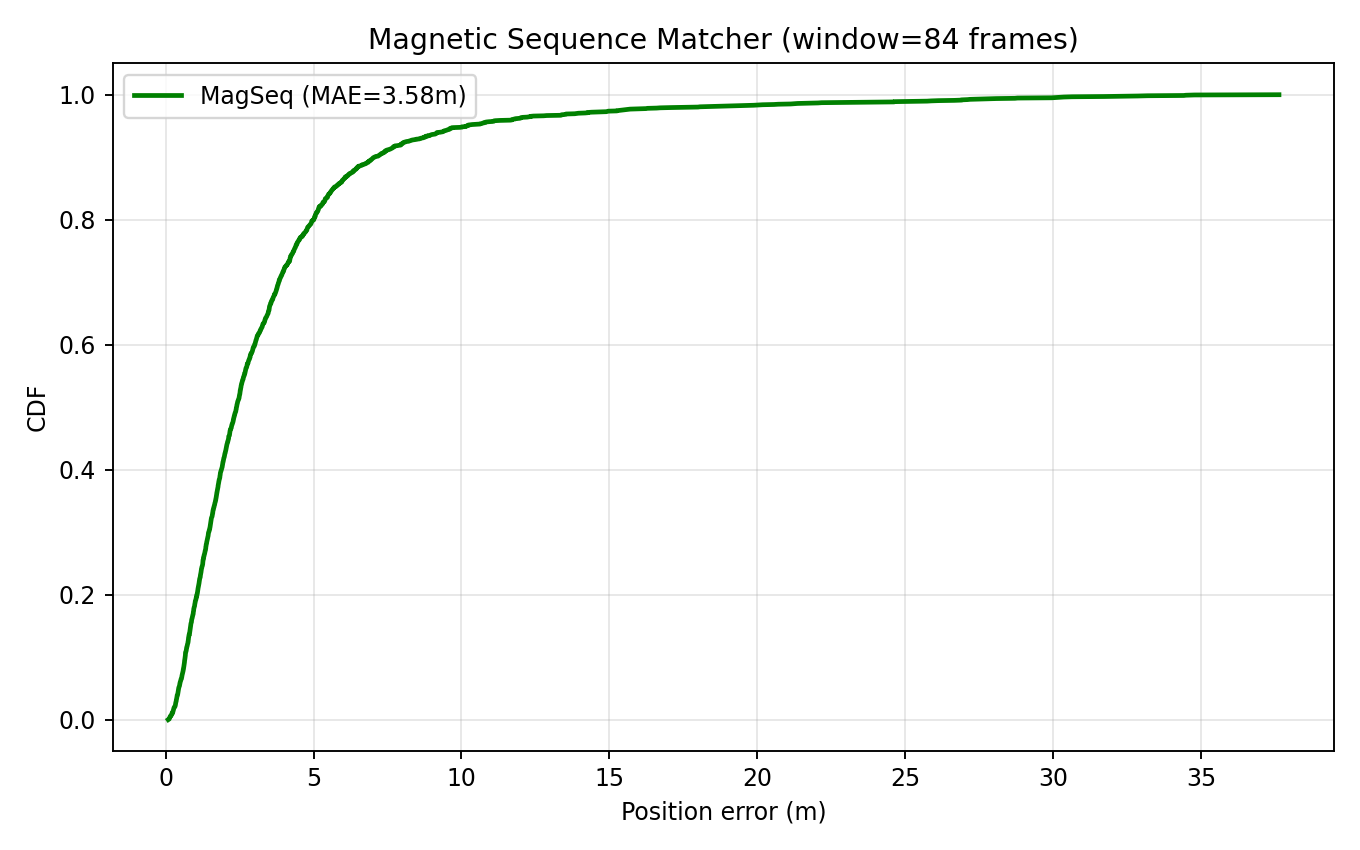
\includegraphics[width=0.85\columnwidth]{mag_cdf_cropped.png}\vspace{0.15cm}
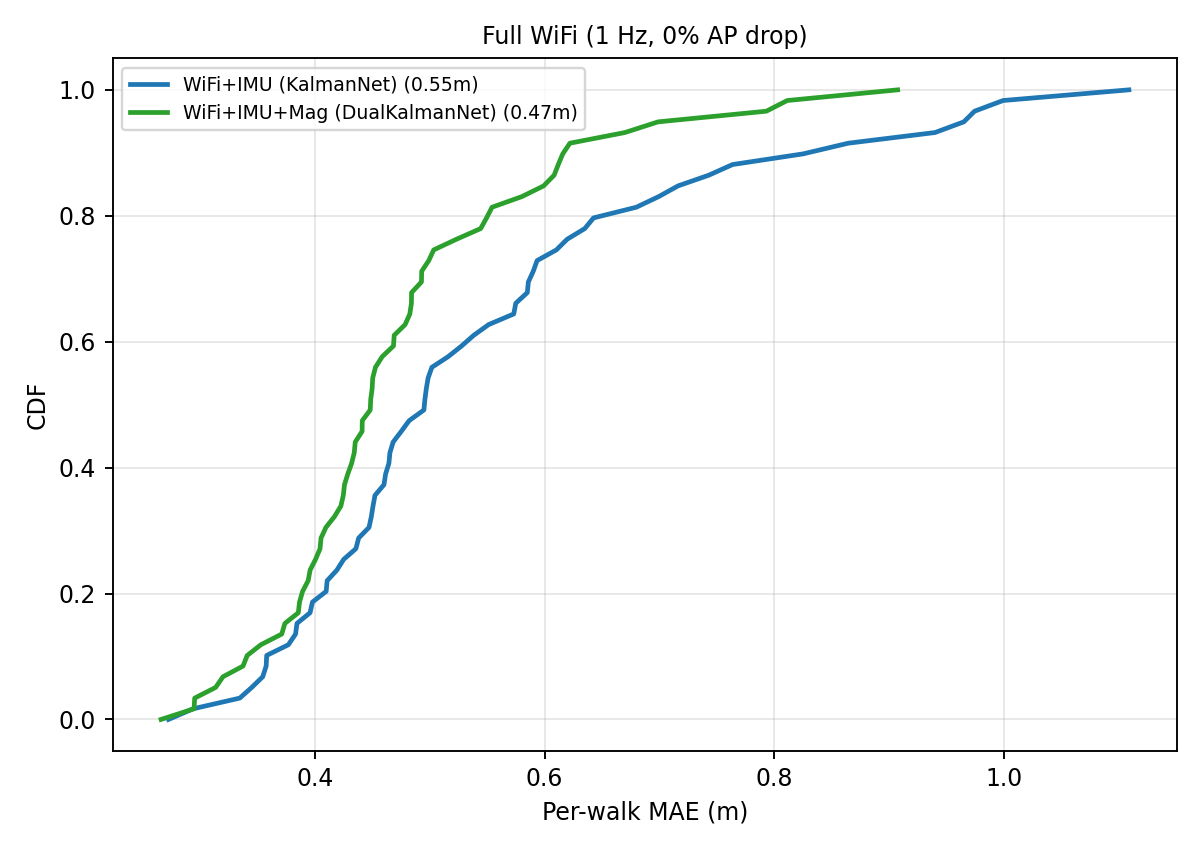
\includegraphics[width=0.85\columnwidth]{kalman_full_wifi.png}\vspace{0.15cm}
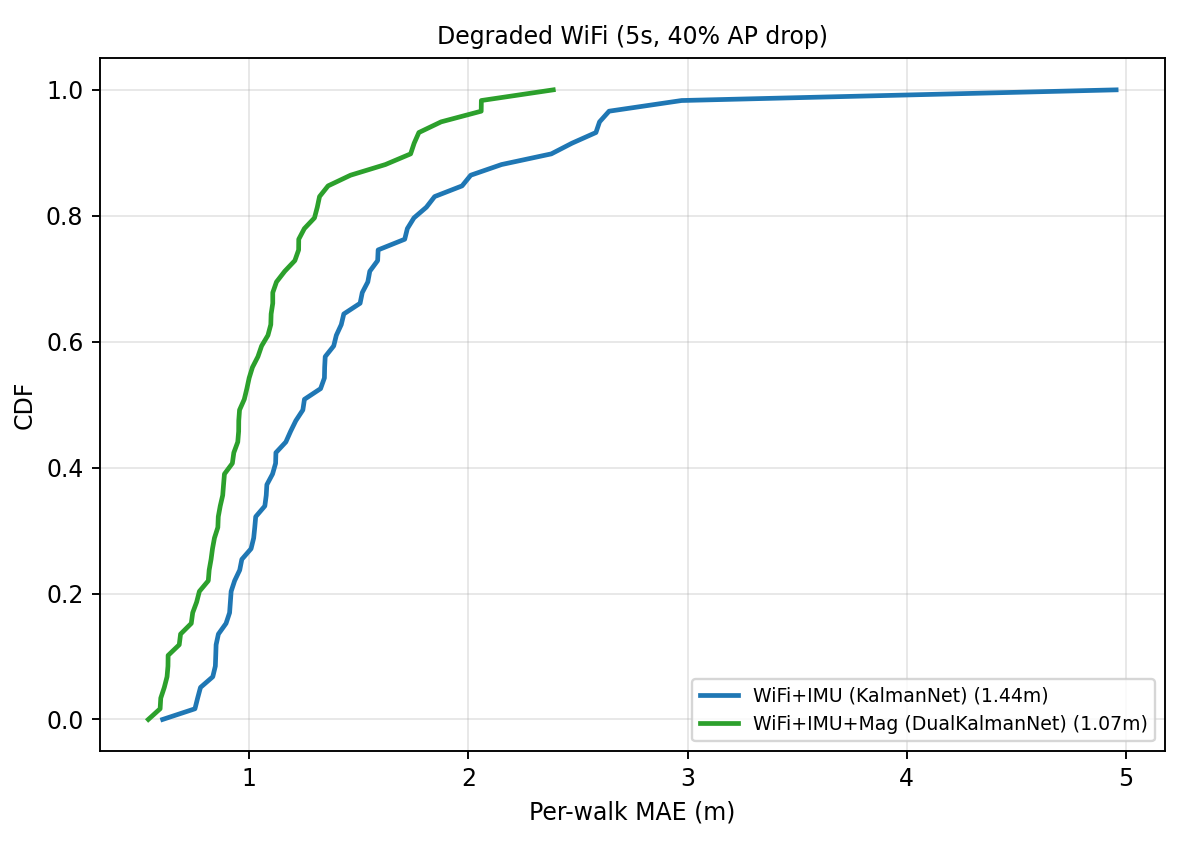
\includegraphics[width=0.85\columnwidth]{kalman_degraded_wifi.png}
\caption{Cumulative Distribution Functions (CDF) of the tracking models. Top: standalone 1D-CNN magnetic sequence matcher error. Middle: Temporal fusion performance under full Wi-Fi conditions (1 Hz). Bottom: Temporal fusion performance under degraded Wi-Fi scenarios (5s gap, 40\% AP dropout), highlighting the significant impact of the magnetic innovation.}
\label{fig:merged_cdfs}
\end{figure}

In standard operating conditions featuring high-frequency 1~Hz Wi-Fi fixes, integrating the continuous magnetic sequence data provides a noticeable 13.4\% improvement in localization accuracy. However, the true strength of the architecture is definitively revealed in the degraded signal regime (Figure~\ref{fig:merged_cdfs}, bottom). When Wi-Fi scans are artificially restricted to one reading every 5 seconds accompanied by a severe 40\% missing AP dropout rate, the classical single-innovation approach drifts significantly. In contrast, the continuous 16.7~Hz magnetic updates act as an effective, dense bridge, yielding a substantial 25.3\% reduction in Mean Absolute Error (improving from 1.44~m to 1.07~m).

\begin{figure}[htbp]
\centering
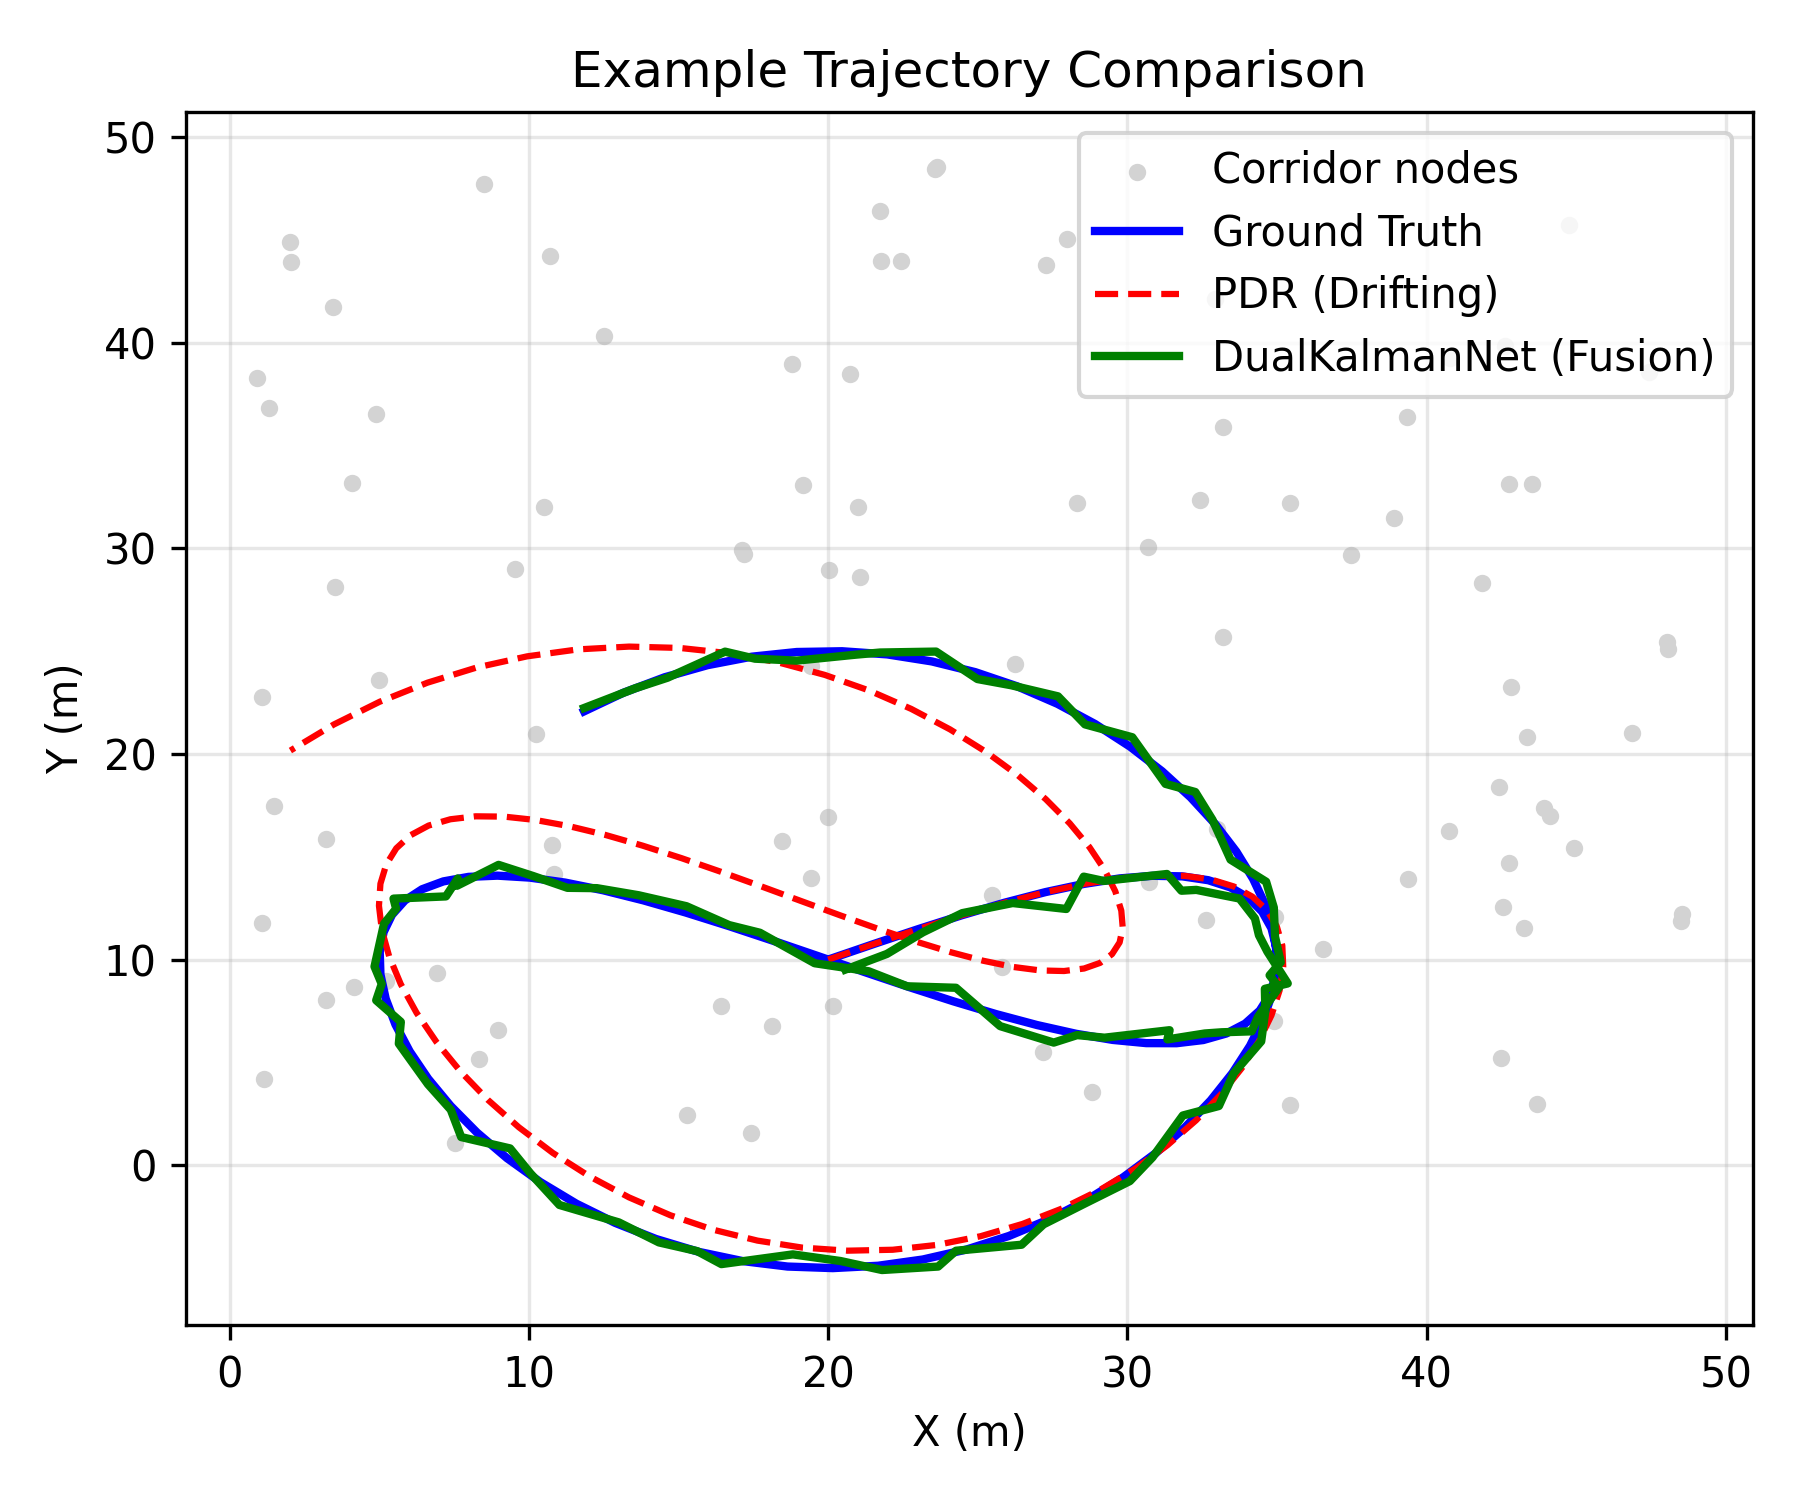
\includegraphics[width=0.9\columnwidth]{trajectory_example.png}
\caption{Example trajectory visualization illustrating tracking divergence. Without frequent Wi-Fi spatial anchors, the standard PDR path (dashed red) drifts due to heading accumulation errors. The Dual-Innovation KalmanNet (solid green) tightly tracks the ground truth (solid blue) by integrating structural magnetic sequence measurements continuously.}
\label{fig:trajectory}
\end{figure}

\subsection{Robustness and Postural Independence}

To validate the generalizability of the framework, the training data intentionally includes three distinct device holding modes present in the MagWi dataset: standard navigation hold, call listening (device near the ear), and natural arm swinging. Because the Wi-Fi MLP operates on scalar RSSI values (orientation-independent) and the magnetic CNN processes rotation-invariant features (field magnitude, vertical/horizontal projections, and dip angle), the architecture is inherently robust to postural variation. This postural agnosticism is critical for real-world deployment where users hold devices in unpredictable orientations.

\section{Conclusion}\label{sec:conclusion}

This paper introduced a generalized, decoupled Neural-Kalman fusion architecture designed to resolve pervasive limitations in deep-learning indoor positioning systems across Hybrid Wi-Fi, Magnetic, and IMU data regimes. By strictly separating spatial inference from temporal tracking modules, the framework successfully circumvents trajectory memorization and orientation-dependent data bias. The integration of a 1D-CNN magnetic sequence matcher alongside an MLP Wi-Fi probability heatmap enables robust spatial updates. Fusing these estimates through an extended KalmanNet architecture enables the system to continuously calculate context-dependent $2\!\times\!2$ matrix gains, leveraging availability masks to maintain resilience against missing sensor modalities.

In challenging, degraded scenarios—a common reality in physical deployments—the dual-innovation system effectively prevents inertial drift, delivering an impressive 25.3\% performance increase over standard models. While current configurations necessitate building-specific training due to unique foundational AP signatures, the mathematical structure is universally applicable. Future research efforts will focus on expanding the architecture to facilitate full three-dimensional, multi-floor positioning by integrating barometric pressure altitude data into the KalmanNet state vector.

\section*{Acknowledgment}
The authors acknowledge the Summer Undergraduate Research Award (SURA) program at the Indian Institute of Technology Delhi for supporting this research.

\bibliographystyle{ieeetr}
\bibliography{Ref}

\end{document}
